% Options for packages loaded elsewhere
\PassOptionsToPackage{unicode}{hyperref}
\PassOptionsToPackage{hyphens}{url}
%
\documentclass[
]{article}
\title{PSTAT174 Final Project}
\author{Joseph Chang}
\date{3/11/2022}

\usepackage{amsmath,amssymb}
\usepackage{lmodern}
\usepackage{iftex}
\ifPDFTeX
  \usepackage[T1]{fontenc}
  \usepackage[utf8]{inputenc}
  \usepackage{textcomp} % provide euro and other symbols
\else % if luatex or xetex
  \usepackage{unicode-math}
  \defaultfontfeatures{Scale=MatchLowercase}
  \defaultfontfeatures[\rmfamily]{Ligatures=TeX,Scale=1}
\fi
% Use upquote if available, for straight quotes in verbatim environments
\IfFileExists{upquote.sty}{\usepackage{upquote}}{}
\IfFileExists{microtype.sty}{% use microtype if available
  \usepackage[]{microtype}
  \UseMicrotypeSet[protrusion]{basicmath} % disable protrusion for tt fonts
}{}
\makeatletter
\@ifundefined{KOMAClassName}{% if non-KOMA class
  \IfFileExists{parskip.sty}{%
    \usepackage{parskip}
  }{% else
    \setlength{\parindent}{0pt}
    \setlength{\parskip}{6pt plus 2pt minus 1pt}}
}{% if KOMA class
  \KOMAoptions{parskip=half}}
\makeatother
\usepackage{xcolor}
\IfFileExists{xurl.sty}{\usepackage{xurl}}{} % add URL line breaks if available
\IfFileExists{bookmark.sty}{\usepackage{bookmark}}{\usepackage{hyperref}}
\hypersetup{
  pdftitle={PSTAT174 Final Project},
  pdfauthor={Joseph Chang},
  hidelinks,
  pdfcreator={LaTeX via pandoc}}
\urlstyle{same} % disable monospaced font for URLs
\usepackage[margin=1in]{geometry}
\usepackage{color}
\usepackage{fancyvrb}
\newcommand{\VerbBar}{|}
\newcommand{\VERB}{\Verb[commandchars=\\\{\}]}
\DefineVerbatimEnvironment{Highlighting}{Verbatim}{commandchars=\\\{\}}
% Add ',fontsize=\small' for more characters per line
\usepackage{framed}
\definecolor{shadecolor}{RGB}{248,248,248}
\newenvironment{Shaded}{\begin{snugshade}}{\end{snugshade}}
\newcommand{\AlertTok}[1]{\textcolor[rgb]{0.94,0.16,0.16}{#1}}
\newcommand{\AnnotationTok}[1]{\textcolor[rgb]{0.56,0.35,0.01}{\textbf{\textit{#1}}}}
\newcommand{\AttributeTok}[1]{\textcolor[rgb]{0.77,0.63,0.00}{#1}}
\newcommand{\BaseNTok}[1]{\textcolor[rgb]{0.00,0.00,0.81}{#1}}
\newcommand{\BuiltInTok}[1]{#1}
\newcommand{\CharTok}[1]{\textcolor[rgb]{0.31,0.60,0.02}{#1}}
\newcommand{\CommentTok}[1]{\textcolor[rgb]{0.56,0.35,0.01}{\textit{#1}}}
\newcommand{\CommentVarTok}[1]{\textcolor[rgb]{0.56,0.35,0.01}{\textbf{\textit{#1}}}}
\newcommand{\ConstantTok}[1]{\textcolor[rgb]{0.00,0.00,0.00}{#1}}
\newcommand{\ControlFlowTok}[1]{\textcolor[rgb]{0.13,0.29,0.53}{\textbf{#1}}}
\newcommand{\DataTypeTok}[1]{\textcolor[rgb]{0.13,0.29,0.53}{#1}}
\newcommand{\DecValTok}[1]{\textcolor[rgb]{0.00,0.00,0.81}{#1}}
\newcommand{\DocumentationTok}[1]{\textcolor[rgb]{0.56,0.35,0.01}{\textbf{\textit{#1}}}}
\newcommand{\ErrorTok}[1]{\textcolor[rgb]{0.64,0.00,0.00}{\textbf{#1}}}
\newcommand{\ExtensionTok}[1]{#1}
\newcommand{\FloatTok}[1]{\textcolor[rgb]{0.00,0.00,0.81}{#1}}
\newcommand{\FunctionTok}[1]{\textcolor[rgb]{0.00,0.00,0.00}{#1}}
\newcommand{\ImportTok}[1]{#1}
\newcommand{\InformationTok}[1]{\textcolor[rgb]{0.56,0.35,0.01}{\textbf{\textit{#1}}}}
\newcommand{\KeywordTok}[1]{\textcolor[rgb]{0.13,0.29,0.53}{\textbf{#1}}}
\newcommand{\NormalTok}[1]{#1}
\newcommand{\OperatorTok}[1]{\textcolor[rgb]{0.81,0.36,0.00}{\textbf{#1}}}
\newcommand{\OtherTok}[1]{\textcolor[rgb]{0.56,0.35,0.01}{#1}}
\newcommand{\PreprocessorTok}[1]{\textcolor[rgb]{0.56,0.35,0.01}{\textit{#1}}}
\newcommand{\RegionMarkerTok}[1]{#1}
\newcommand{\SpecialCharTok}[1]{\textcolor[rgb]{0.00,0.00,0.00}{#1}}
\newcommand{\SpecialStringTok}[1]{\textcolor[rgb]{0.31,0.60,0.02}{#1}}
\newcommand{\StringTok}[1]{\textcolor[rgb]{0.31,0.60,0.02}{#1}}
\newcommand{\VariableTok}[1]{\textcolor[rgb]{0.00,0.00,0.00}{#1}}
\newcommand{\VerbatimStringTok}[1]{\textcolor[rgb]{0.31,0.60,0.02}{#1}}
\newcommand{\WarningTok}[1]{\textcolor[rgb]{0.56,0.35,0.01}{\textbf{\textit{#1}}}}
\usepackage{graphicx}
\makeatletter
\def\maxwidth{\ifdim\Gin@nat@width>\linewidth\linewidth\else\Gin@nat@width\fi}
\def\maxheight{\ifdim\Gin@nat@height>\textheight\textheight\else\Gin@nat@height\fi}
\makeatother
% Scale images if necessary, so that they will not overflow the page
% margins by default, and it is still possible to overwrite the defaults
% using explicit options in \includegraphics[width, height, ...]{}
\setkeys{Gin}{width=\maxwidth,height=\maxheight,keepaspectratio}
% Set default figure placement to htbp
\makeatletter
\def\fps@figure{htbp}
\makeatother
\setlength{\emergencystretch}{3em} % prevent overfull lines
\providecommand{\tightlist}{%
  \setlength{\itemsep}{0pt}\setlength{\parskip}{0pt}}
\setcounter{secnumdepth}{-\maxdimen} % remove section numbering
\ifLuaTeX
  \usepackage{selnolig}  % disable illegal ligatures
\fi

\begin{document}
\maketitle

\begin{Shaded}
\begin{Highlighting}[]
\FunctionTok{library}\NormalTok{(knitr)}
\FunctionTok{library}\NormalTok{(tidyverse) }
\FunctionTok{library}\NormalTok{(ISLR) }
\FunctionTok{library}\NormalTok{(ROCR)}
\FunctionTok{library}\NormalTok{(dplyr)}
\FunctionTok{library}\NormalTok{(tinytex)}
\FunctionTok{library}\NormalTok{(MASS)}
\CommentTok{\#devtools::install\_github("FinYang/tsdl")}
\FunctionTok{library}\NormalTok{(tsdl)}
\FunctionTok{library}\NormalTok{(forecast)}
\FunctionTok{library}\NormalTok{(astsa)}
\FunctionTok{library}\NormalTok{(qpcR)}
\end{Highlighting}
\end{Shaded}

\hypertarget{executive-summary}{%
\section{Executive Summary}\label{executive-summary}}

This project focuses on the United States' defense budget from the years
1960 \textasciitilde{} 2021. The goal of this project is to create a
time series model that could predict the last 10 years (2012-2021) of
the U.S. Defense Budget and compare it with last 10 years (2012-2021)
given by the actual data. In order to do this, I began by splitting the
original dataset into testing and training sets, with training as the
first 51 points and testing as the last 10 points. After training, I
made any necessary transformations using Boxcox and discovered that I
needed to transform the training data by taking its log. Next, when I
differenced and found the smallest variance, I needed to difference the
log of training at lag 1 once. From there, I could plot the ACF and PACF
of my training data and estimate the parameters of a potential model
using a for loop. After model estimation, I considered the two best
models from the lowest AICc and began model diagnostics. In this step, I
tested if the residuals in my candidate models were independent, had any
nonlinear dependence, and were normal. If passed, the model could be
considered for forecasting. In the model forecasting, I predicted the 10
future observations from my best model and concluded that my model
closely followed the actual model for about the first seven points
(years), but then began to diverge from the actual model the rest of the
way. As a final step, I predicted 5 extra years from my predicted model
onto the original dataset just for my curiosity. From this project, I
learned that the United States government spends a tremendous amount of
money (billions of dollars) on its defense budget.

\hypertarget{introduction}{%
\section{Introduction}\label{introduction}}

The data I used shows the United States military defense budget since
1960. The data has a yearly frequency and measures budget spending in
terms of billions of USD. Using the website Kaggle, I imported a csv
file into RStudios and began to analyze the time series data. Although
the original dataset has two other columns dedicated to population and
GDP of US for each respective year, I find the defense budget most
interesting because it matches closely with the history of the United
States and the wars it has participated in. For example, after the fall
of the USSR (1992) and ending the Cold War, US defense spending dipped,
and stayed constant. But after the September 11th attack (2001), total
spending increased exponentially as the government prioritized
protecting its own citizens. Both of these historical events are
corroborated by the data. Thus, the goal of this project is to create a
prediction model that could predict as close to possible of future US
defense spending. To solve this problem, I split training and testing
sets from the original model, with testing as the last 10 points. Using
the training set to predict parameters in my model, I could correctly
determine the best model that would represent the training dataset. In
the forecasting step, I plotted a time series on the training set and
predicted 15 steps ahead: 10 for comparison with testing (marked in red)
and 5 just for my pleasure (marked in blue). Along with these points
were 95 percent confidence intervals that showed the margin of error for
the predicted points. Both the predicted points and confidence intervals
are in blue to signify prediction. The results indicated that the
confidence intervals were very wide, meaning the margin of error could
be large. While the first 7 predicted points were closely related to the
first 7 actual points, the rest of the predicted model showed a very
different trend compared to the testing set. I can conclude that if my
model were to continue predicting beyond the testing set, it would
probably not be very accurate.

\hypertarget{data-importation}{%
\section{Data Importation}\label{data-importation}}

First, I read in the data and plotted the time series model for the
Defense Budget for each of the years, along with a red line for trend
and blue line for mean. Additionally, I created a histogram to visualize
the entire Defense Budget dataset.

\begin{Shaded}
\begin{Highlighting}[]
\NormalTok{spending\_data }\OtherTok{\textless{}{-}} \FunctionTok{read.csv}\NormalTok{(}\StringTok{"/Users/josephchang/Desktop/MilitarySpending.csv.xls"}\NormalTok{)}

\CommentTok{\# added line for trend }
\FunctionTok{plot.ts}\NormalTok{(spending\_data}\SpecialCharTok{$}\NormalTok{DefenseBudget, }\AttributeTok{ylab =} \StringTok{"Defense budget (in US billion)"}\NormalTok{, }\AttributeTok{xlab =} \StringTok{"Year after 1960"}\NormalTok{)}
\NormalTok{nt }\OtherTok{=} \FunctionTok{length}\NormalTok{(spending\_data}\SpecialCharTok{$}\NormalTok{DefenseBudget)}
\NormalTok{fit }\OtherTok{\textless{}{-}} \FunctionTok{lm}\NormalTok{(spending\_data}\SpecialCharTok{$}\NormalTok{DefenseBudget }\SpecialCharTok{\textasciitilde{}} \FunctionTok{as.numeric}\NormalTok{(}\DecValTok{1}\SpecialCharTok{:}\NormalTok{nt))}
\FunctionTok{abline}\NormalTok{(fit, }\AttributeTok{col =}\StringTok{"red"}\NormalTok{)}
\CommentTok{\# added mean}
\NormalTok{data\_mean }\OtherTok{\textless{}{-}} \FunctionTok{mean}\NormalTok{(spending\_data}\SpecialCharTok{$}\NormalTok{DefenseBudget)}
\FunctionTok{abline}\NormalTok{(}\AttributeTok{h=}\NormalTok{data\_mean, }\AttributeTok{col=}\StringTok{"blue"}\NormalTok{)}
\end{Highlighting}
\end{Shaded}

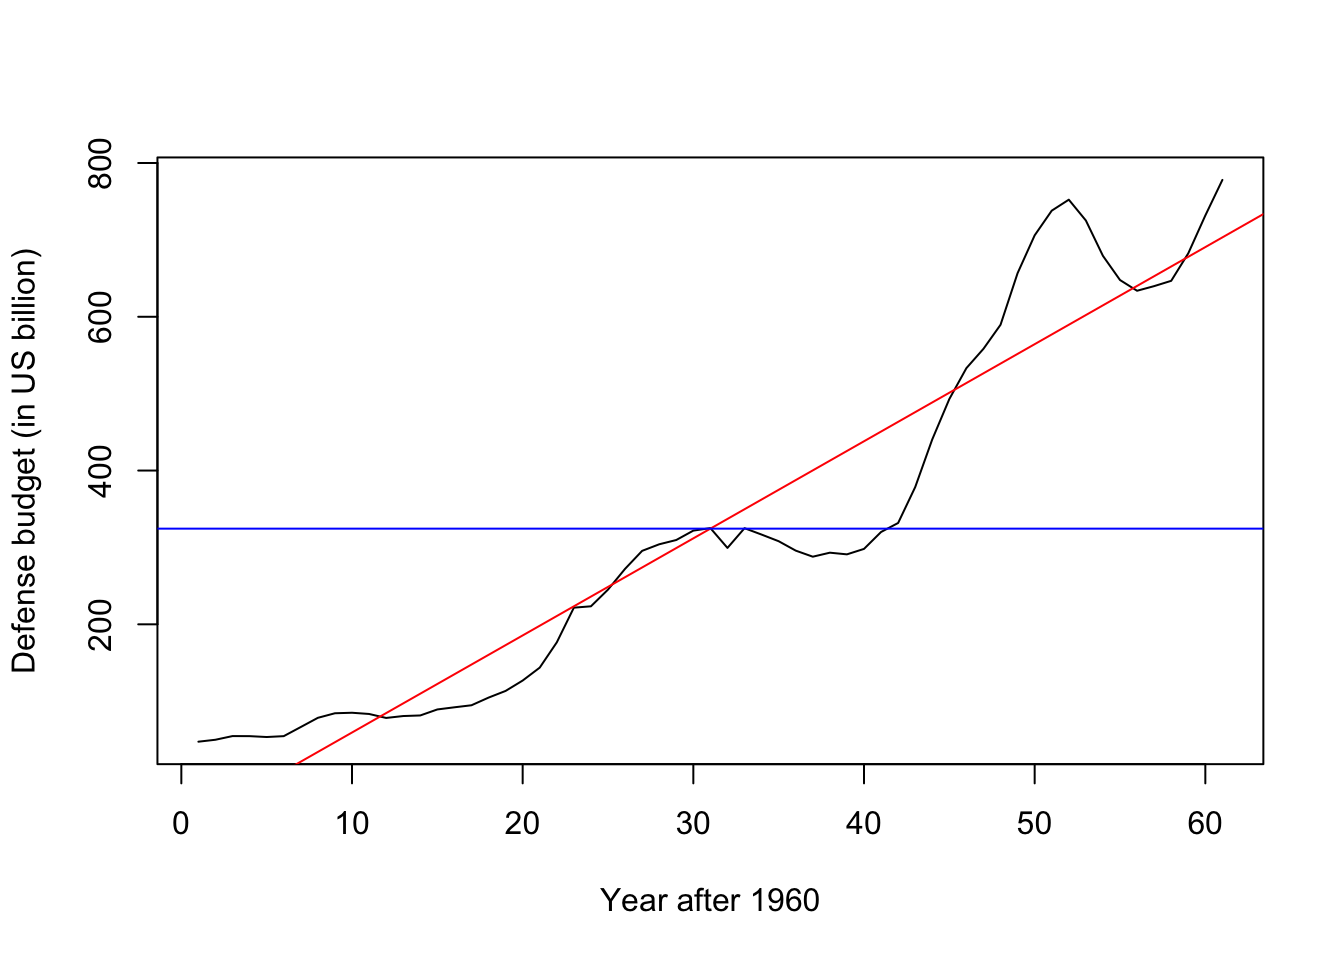
\includegraphics{Joseph-Chang---PSTAT174-Final-Project_files/figure-latex/unnamed-chunk-2-1.pdf}

\begin{Shaded}
\begin{Highlighting}[]
\CommentTok{\# histogram of original data points}
\FunctionTok{hist}\NormalTok{(spending\_data}\SpecialCharTok{$}\NormalTok{DefenseBudget, }\AttributeTok{label=}\ConstantTok{TRUE}\NormalTok{, }\AttributeTok{main =} \StringTok{"Histogram of U.S Defense Budget"}\NormalTok{, }\AttributeTok{breaks=}\StringTok{"Sturges"}\NormalTok{, }\AttributeTok{xlab =} \StringTok{"Defense Budget (in US billion)"}\NormalTok{)}
\end{Highlighting}
\end{Shaded}

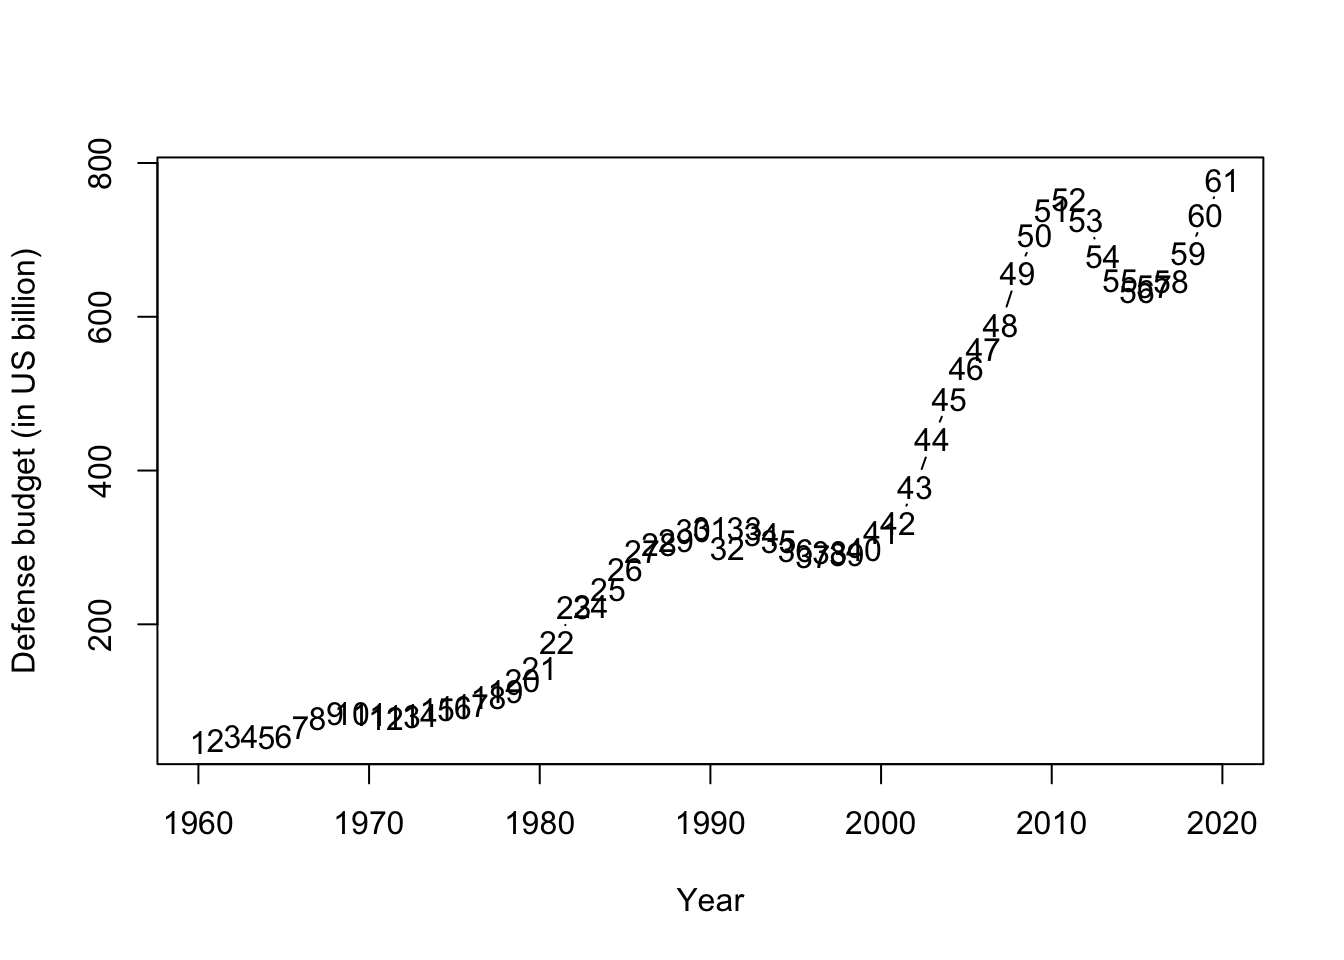
\includegraphics{Joseph-Chang---PSTAT174-Final-Project_files/figure-latex/unnamed-chunk-2-2.pdf}

Immediate observations: There seems to be a linear trend that is
positive but there is no seasonality and no apparent sharp change in
behavior. There is non-constant variance and mean, where mean is 324.4
billion USD. The histogram seems to be skewed right.

\hypertarget{testing-and-training-for-the-original-data}{%
\section{Testing and training for the original
data}\label{testing-and-training-for-the-original-data}}

Next, I created training and testing sets from the original data. For
better visualization, I plotted the time series plot for the training
set, along with trend in red and mean in blue. In addition, I plotted a
histogram of the training set.

\begin{Shaded}
\begin{Highlighting}[]
\CommentTok{\# Define training and testing sets}
\NormalTok{training }\OtherTok{=}\NormalTok{ spending\_data}\SpecialCharTok{$}\NormalTok{DefenseBudget[}\FunctionTok{c}\NormalTok{(}\DecValTok{1}\SpecialCharTok{:}\DecValTok{51}\NormalTok{)]}
\NormalTok{testing  }\OtherTok{=}\NormalTok{ spending\_data}\SpecialCharTok{$}\NormalTok{DefenseBudget[}\FunctionTok{c}\NormalTok{(}\DecValTok{52}\SpecialCharTok{:}\DecValTok{61}\NormalTok{)]}

\CommentTok{\# time series plot in training with trend and mean}
\FunctionTok{plot.ts}\NormalTok{(training, }\AttributeTok{ylab =} \StringTok{"Defense budget (in US billion)"}\NormalTok{, }\AttributeTok{xlab =} \StringTok{"Year after 1960"}\NormalTok{)}
\NormalTok{fit }\OtherTok{\textless{}{-}} \FunctionTok{lm}\NormalTok{(training }\SpecialCharTok{\textasciitilde{}} \FunctionTok{as.numeric}\NormalTok{(}\DecValTok{1}\SpecialCharTok{:}\FunctionTok{length}\NormalTok{(training)))}
\FunctionTok{abline}\NormalTok{(fit, }\AttributeTok{col=}\StringTok{"red"}\NormalTok{)}
\FunctionTok{abline}\NormalTok{(}\AttributeTok{h=}\FunctionTok{mean}\NormalTok{(training), }\AttributeTok{col =} \StringTok{"blue"}\NormalTok{)}
\end{Highlighting}
\end{Shaded}

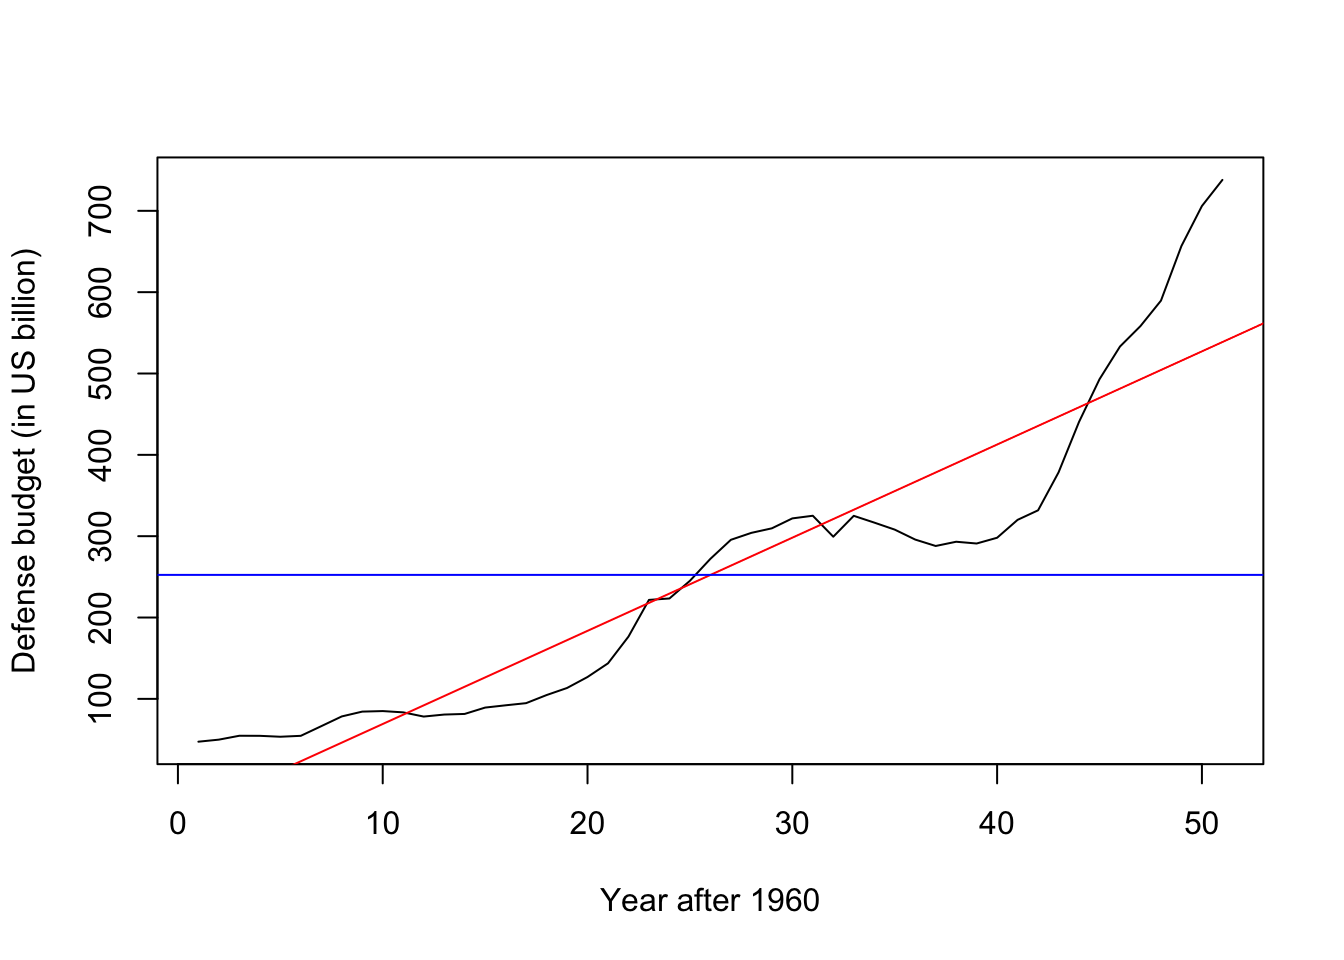
\includegraphics{Joseph-Chang---PSTAT174-Final-Project_files/figure-latex/unnamed-chunk-3-1.pdf}

\begin{Shaded}
\begin{Highlighting}[]
\CommentTok{\# histogram of original data points}
\FunctionTok{hist}\NormalTok{(training, }\AttributeTok{label=}\ConstantTok{TRUE}\NormalTok{, }\AttributeTok{main =} \StringTok{"Histogram of training set of U.S Defense Budget"}\NormalTok{, }\AttributeTok{breaks=}\StringTok{"Sturges"}\NormalTok{, }\AttributeTok{xlab =} \StringTok{"Defense Budget (in US billion)"}\NormalTok{)}
\end{Highlighting}
\end{Shaded}

\includegraphics{Joseph-Chang---PSTAT174-Final-Project_files/figure-latex/unnamed-chunk-3-2.pdf}

Based from the original data and training data, both look about the
same. The training data appears to have a linear positive trend with no
seasonality or sharpe changes. There is still non-constant variance and
mean, where mean is now 252.4 billion USD. The histogram still looks
skewed right.

\hypertarget{transformation}{%
\section{Transformation}\label{transformation}}

Next, since the original data looked skewed, I will see if I need to
make any necessary transformations to make the model stationary and to
stabilize the variance.

\begin{Shaded}
\begin{Highlighting}[]
\NormalTok{t }\OtherTok{\textless{}{-}} \DecValTok{1}\SpecialCharTok{:}\FunctionTok{length}\NormalTok{(training)}
\NormalTok{fit }\OtherTok{\textless{}{-}} \FunctionTok{lm}\NormalTok{(training}\SpecialCharTok{\textasciitilde{}}\NormalTok{t)}
\NormalTok{bcTransform }\OtherTok{\textless{}{-}} \FunctionTok{boxcox}\NormalTok{(training }\SpecialCharTok{\textasciitilde{}}\NormalTok{ t, }\AttributeTok{plotit=}\ConstantTok{TRUE}\NormalTok{)}
\end{Highlighting}
\end{Shaded}

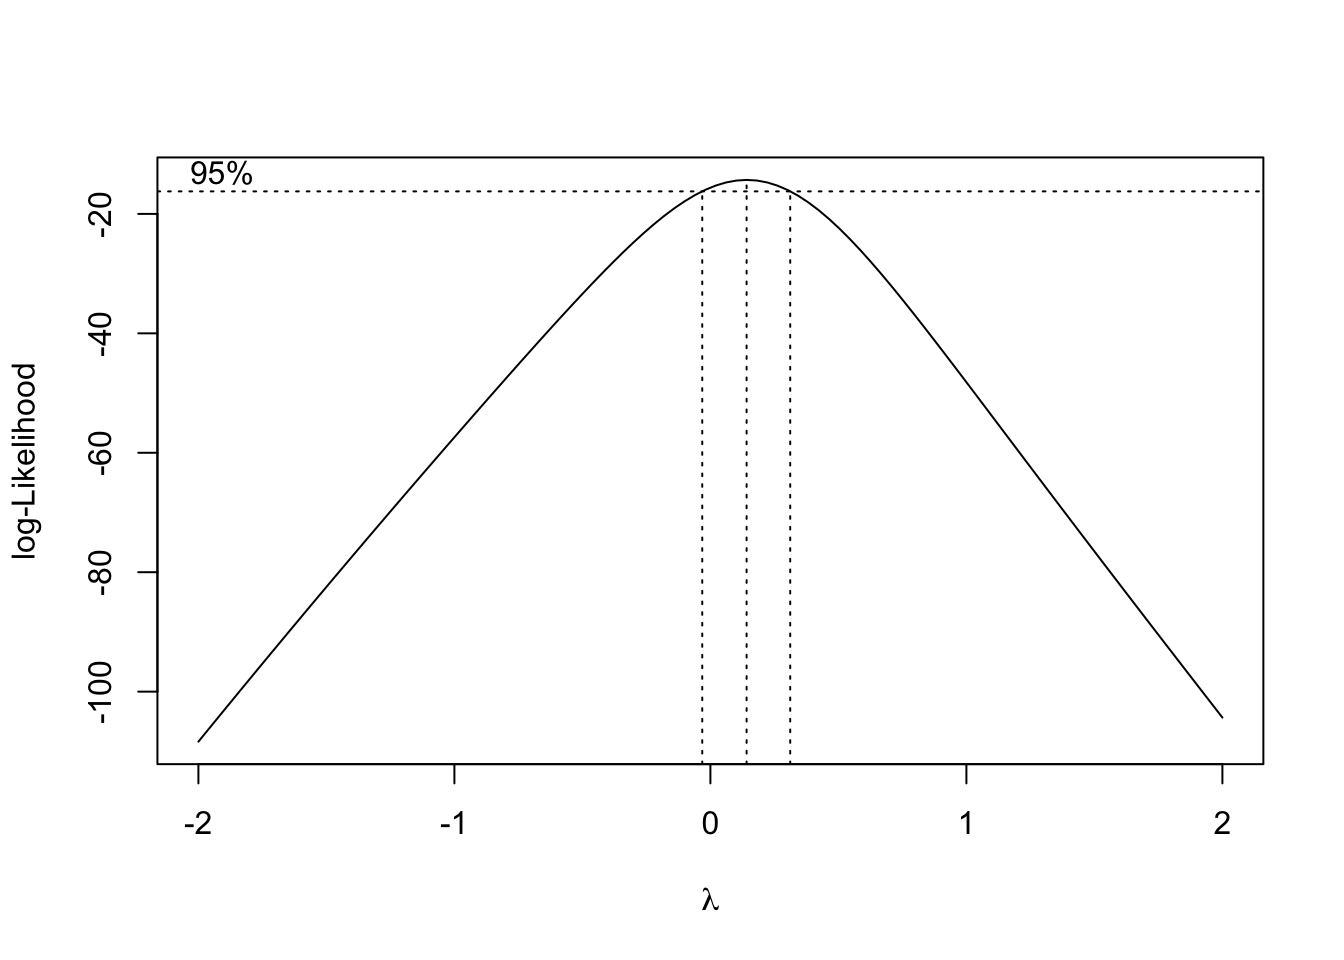
\includegraphics{Joseph-Chang---PSTAT174-Final-Project_files/figure-latex/unnamed-chunk-4-1.pdf}

\begin{Shaded}
\begin{Highlighting}[]
\NormalTok{lambda }\OtherTok{=}\NormalTok{ bcTransform}\SpecialCharTok{$}\NormalTok{x[}\FunctionTok{which}\NormalTok{(bcTransform}\SpecialCharTok{$}\NormalTok{y }\SpecialCharTok{==} \FunctionTok{max}\NormalTok{(bcTransform}\SpecialCharTok{$}\NormalTok{y))]}
\end{Highlighting}
\end{Shaded}

Using the Box-Cox transformation, the BcTransform command gave me the
value of lambda to be around 0.1414. Thus, I named the box-cox
transformation data as training.bc. One thing I do notice that 0 is
inside the confidence interval, so a log transformation is another
possibility. As such, I will define it as training.log.

\begin{Shaded}
\begin{Highlighting}[]
\CommentTok{\# define boxcox transformation and log transformation for training set}
\NormalTok{training.bc }\OtherTok{=}\NormalTok{ (}\DecValTok{1}\SpecialCharTok{/}\NormalTok{lambda)}\SpecialCharTok{*}\NormalTok{(training}\SpecialCharTok{\^{}}\NormalTok{lambda}\DecValTok{{-}1}\NormalTok{)}
\NormalTok{training.log }\OtherTok{=} \FunctionTok{log}\NormalTok{(training)}
\end{Highlighting}
\end{Shaded}

In order to determine which model to use, I will create time series
plots for training, box-cox transformation, and log transformation. I
will create histograms of each as well.

\begin{Shaded}
\begin{Highlighting}[]
\CommentTok{\# compare transforms on time series plot}
\NormalTok{op}\OtherTok{=}\FunctionTok{par}\NormalTok{(}\AttributeTok{mfrow=}\FunctionTok{c}\NormalTok{(}\DecValTok{2}\NormalTok{,}\DecValTok{2}\NormalTok{))}
\FunctionTok{plot.ts}\NormalTok{(training, }\AttributeTok{main =} \StringTok{"Original Training set"}\NormalTok{)}
\FunctionTok{plot.ts}\NormalTok{(training.bc, }\AttributeTok{main =} \StringTok{"Box{-}cox Transform"}\NormalTok{)}
\FunctionTok{plot.ts}\NormalTok{(training.log, }\AttributeTok{main =} \StringTok{"Log Transform"}\NormalTok{)}

\CommentTok{\# compare transforms on histogram}
\NormalTok{op}\OtherTok{=}\FunctionTok{par}\NormalTok{(}\AttributeTok{mfrow=}\FunctionTok{c}\NormalTok{(}\DecValTok{2}\NormalTok{,}\DecValTok{2}\NormalTok{))}
\end{Highlighting}
\end{Shaded}

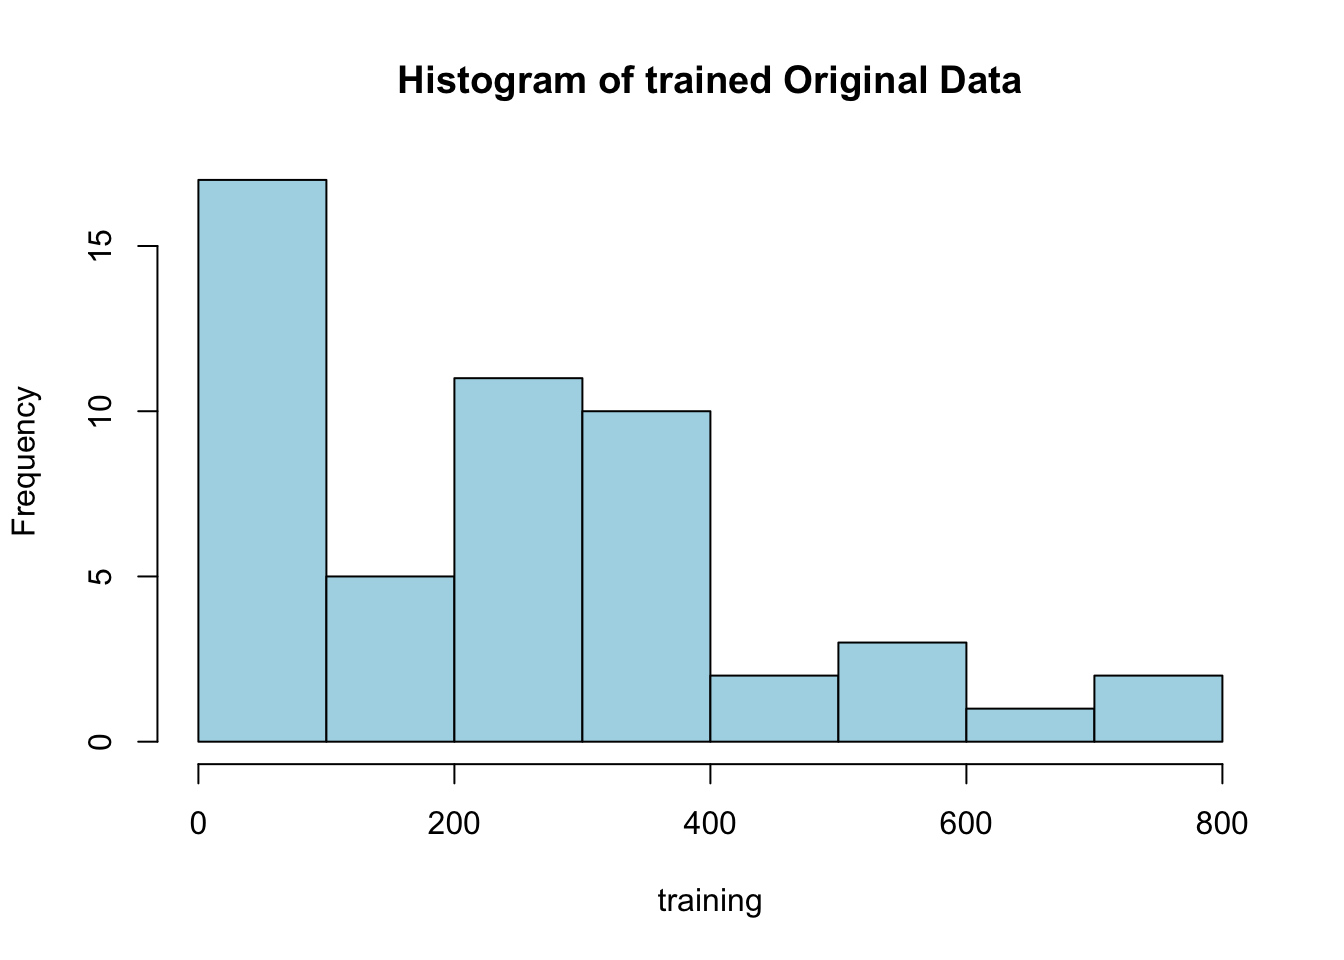
\includegraphics{Joseph-Chang---PSTAT174-Final-Project_files/figure-latex/unnamed-chunk-6-1.pdf}

\begin{Shaded}
\begin{Highlighting}[]
\FunctionTok{hist}\NormalTok{(training, }\AttributeTok{col =} \StringTok{"light blue"}\NormalTok{, }\AttributeTok{main =} \StringTok{"Histogram of trained Original Data"}\NormalTok{, }\AttributeTok{breaks =} \StringTok{"Sturges"}\NormalTok{)}
\FunctionTok{hist}\NormalTok{(training.bc, }\AttributeTok{col =} \StringTok{"light blue"}\NormalTok{, }\AttributeTok{main =} \StringTok{"Histogram of Boxcox transformed Data"}\NormalTok{, }\AttributeTok{breaks=}\StringTok{"Sturges"}\NormalTok{)}
\FunctionTok{hist}\NormalTok{(training.log, }\AttributeTok{col =} \StringTok{"light blue"}\NormalTok{, }\AttributeTok{main =} \StringTok{"Histogram of Log transformed Data"}\NormalTok{, }\AttributeTok{breaks=}\StringTok{"Sturges"}\NormalTok{)}
\end{Highlighting}
\end{Shaded}

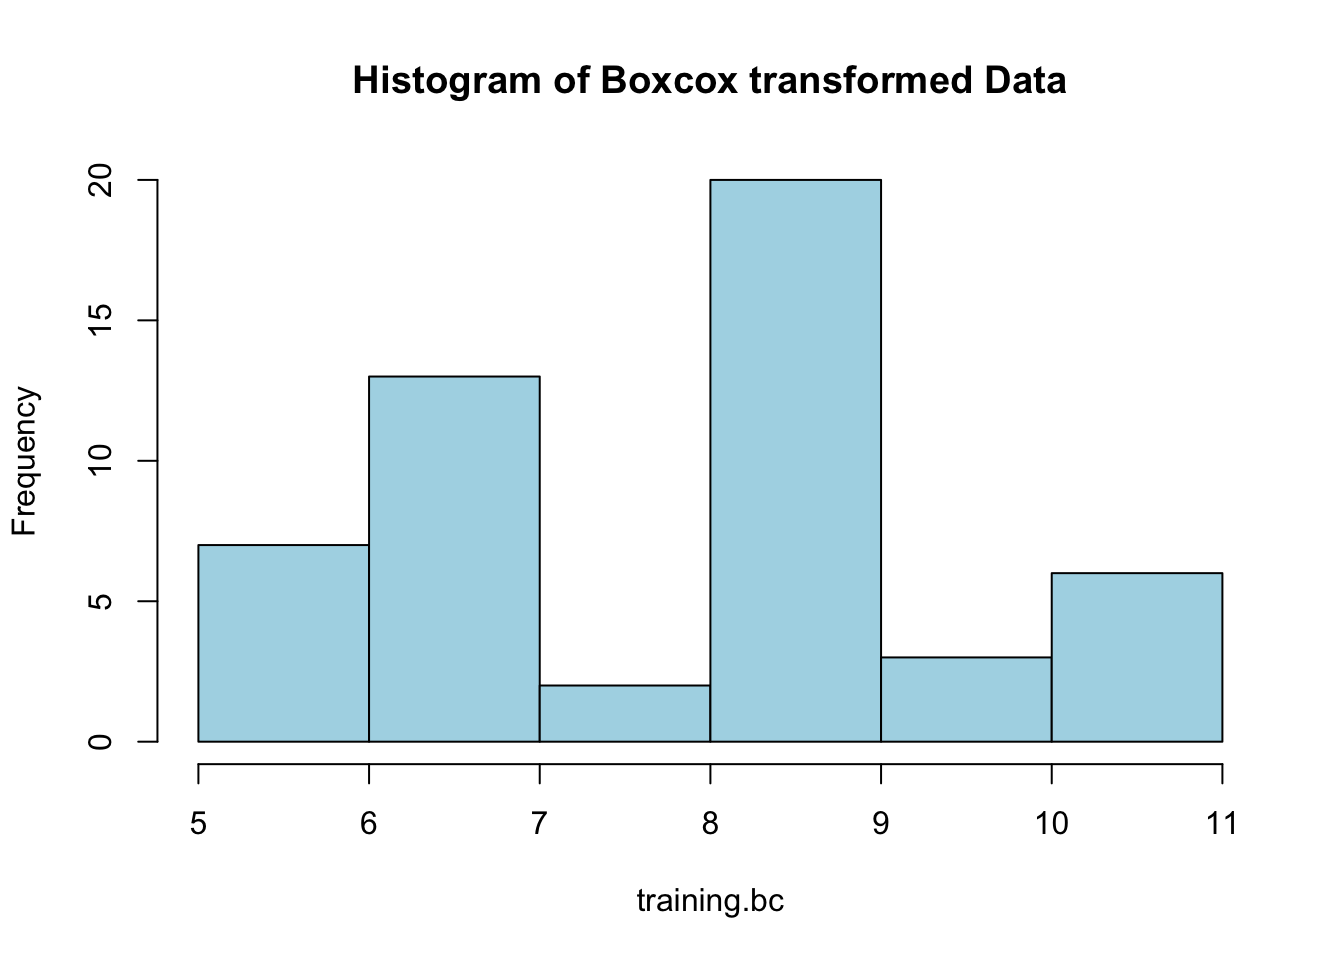
\includegraphics{Joseph-Chang---PSTAT174-Final-Project_files/figure-latex/unnamed-chunk-6-2.pdf}

From the time series plot, the both the box-cox transform and the log
transform look to have a more stable variance and trend than the
original. Based from the histogram, the original is still looking skewed
right while the box-cox transformation looks more symmetric. Log
transformation looks even more symmetric than the box-cox. As a result,
the log transformation looks the most appropriate to use based on my
judgement.

\hypertarget{differencing}{%
\section{Differencing}\label{differencing}}

Then, I want to check if training.log needed any differencing to remove
trend. To begin, I differenced once the log of training set at lag 1,
when d=2, and d=3. All differencing took place at lag 1. Additionally, I
checked the variances of each time I differenced as well.

\begin{Shaded}
\begin{Highlighting}[]
\NormalTok{dat}\FloatTok{.1} \OtherTok{\textless{}{-}} \FunctionTok{diff}\NormalTok{(training.log, }\DecValTok{1}\NormalTok{)}
\NormalTok{dat}\FloatTok{.2} \OtherTok{\textless{}{-}} \FunctionTok{diff}\NormalTok{(dat}\FloatTok{.1}\NormalTok{, }\DecValTok{1}\NormalTok{)}
\NormalTok{dat}\FloatTok{.3} \OtherTok{\textless{}{-}} \FunctionTok{diff}\NormalTok{(dat}\FloatTok{.2}\NormalTok{, }\DecValTok{1}\NormalTok{)}

\CommentTok{\# check variances}
\FunctionTok{var}\NormalTok{(training.log)}
\end{Highlighting}
\end{Shaded}

\begin{verbatim}
## [1] 0.6646
\end{verbatim}

\begin{Shaded}
\begin{Highlighting}[]
\FunctionTok{var}\NormalTok{(dat}\FloatTok{.1}\NormalTok{)}
\end{Highlighting}
\end{Shaded}

\begin{verbatim}
## [1] 0.00457
\end{verbatim}

\begin{Shaded}
\begin{Highlighting}[]
\FunctionTok{var}\NormalTok{(dat}\FloatTok{.2}\NormalTok{)}
\end{Highlighting}
\end{Shaded}

\begin{verbatim}
## [1] 0.004732
\end{verbatim}

\begin{Shaded}
\begin{Highlighting}[]
\FunctionTok{var}\NormalTok{(dat}\FloatTok{.3}\NormalTok{)}
\end{Highlighting}
\end{Shaded}

\begin{verbatim}
## [1] 0.01196
\end{verbatim}

Based from the variances, I only need to difference when d=1 because
variance is lowest when d=1. At d=2, variance increased again.
Therefore, d=1 is most appropriate.

Therefore, I plotted the time series for dat.1 along with its mean
colored in blue as well as its histogram.

\begin{Shaded}
\begin{Highlighting}[]
\CommentTok{\# time series plot for dat.1}
\FunctionTok{plot.ts}\NormalTok{(dat}\FloatTok{.1}\NormalTok{, }\AttributeTok{main =} \StringTok{"log training when d=1"}\NormalTok{, }\AttributeTok{type=} \StringTok{"l"}\NormalTok{)}
\NormalTok{fit\_a }\OtherTok{\textless{}{-}} \FunctionTok{lm}\NormalTok{(dat}\FloatTok{.1} \SpecialCharTok{\textasciitilde{}} \FunctionTok{as.numeric}\NormalTok{(}\DecValTok{1}\SpecialCharTok{:}\FunctionTok{length}\NormalTok{(dat}\FloatTok{.1}\NormalTok{)))}
\FunctionTok{abline}\NormalTok{(fit\_a, }\AttributeTok{col =} \StringTok{"red"}\NormalTok{)}
\FunctionTok{abline}\NormalTok{(}\AttributeTok{h=}\FunctionTok{mean}\NormalTok{(dat}\FloatTok{.1}\NormalTok{), }\AttributeTok{col =} \StringTok{"blue"}\NormalTok{)}
\end{Highlighting}
\end{Shaded}

\includegraphics{Joseph-Chang---PSTAT174-Final-Project_files/figure-latex/unnamed-chunk-8-1.pdf}

\begin{Shaded}
\begin{Highlighting}[]
\CommentTok{\# histogram of dat.1}
\FunctionTok{hist}\NormalTok{(dat}\FloatTok{.1}\NormalTok{, }\AttributeTok{col =} \StringTok{"light blue"}\NormalTok{, }\AttributeTok{xlab =} \StringTok{""}\NormalTok{, }\AttributeTok{main =} \StringTok{"Histogram at d=1"}\NormalTok{)}
\NormalTok{m }\OtherTok{\textless{}{-}} \FunctionTok{mean}\NormalTok{(dat}\FloatTok{.2}\NormalTok{)}
\NormalTok{std }\OtherTok{\textless{}{-}} \FunctionTok{sqrt}\NormalTok{(}\FunctionTok{var}\NormalTok{(dat}\FloatTok{.2}\NormalTok{))}
\FunctionTok{curve}\NormalTok{(}\FunctionTok{dnorm}\NormalTok{(x,m,std), }\AttributeTok{add =}\NormalTok{ T)}
\end{Highlighting}
\end{Shaded}

\includegraphics{Joseph-Chang---PSTAT174-Final-Project_files/figure-latex/unnamed-chunk-8-2.pdf}

The time series plot for dat.1 looks somewhat stationary and the
histogram looks somewhat gaussian, but overall maybe skewed left.

\hypertarget{model-identification}{%
\section{Model Identification}\label{model-identification}}

For comparison, I plotted ACF and PACF for dat.1. I set the maximum lag
at 40 because since there is no seasonality in training, I won't need an
more data than I need.

\begin{Shaded}
\begin{Highlighting}[]
\CommentTok{\# ACF and PACF for dat.1}
\NormalTok{op }\OtherTok{\textless{}{-}} \FunctionTok{par}\NormalTok{(}\AttributeTok{no.readonly=}\ConstantTok{TRUE}\NormalTok{)}
\FunctionTok{acf}\NormalTok{(dat}\FloatTok{.1}\NormalTok{, }\AttributeTok{lag.max =} \DecValTok{40}\NormalTok{, }\AttributeTok{main=}\StringTok{"ACF of difference at lag 1 once"}\NormalTok{, }\AttributeTok{ylim=}\FunctionTok{c}\NormalTok{(}\SpecialCharTok{{-}}\DecValTok{1}\NormalTok{,}\DecValTok{1}\NormalTok{),}\AttributeTok{xlab=}\StringTok{"h"}\NormalTok{, }\AttributeTok{ylab=} \FunctionTok{expression}\NormalTok{(}\FunctionTok{hat}\NormalTok{(rho)[X](h)))}
\end{Highlighting}
\end{Shaded}

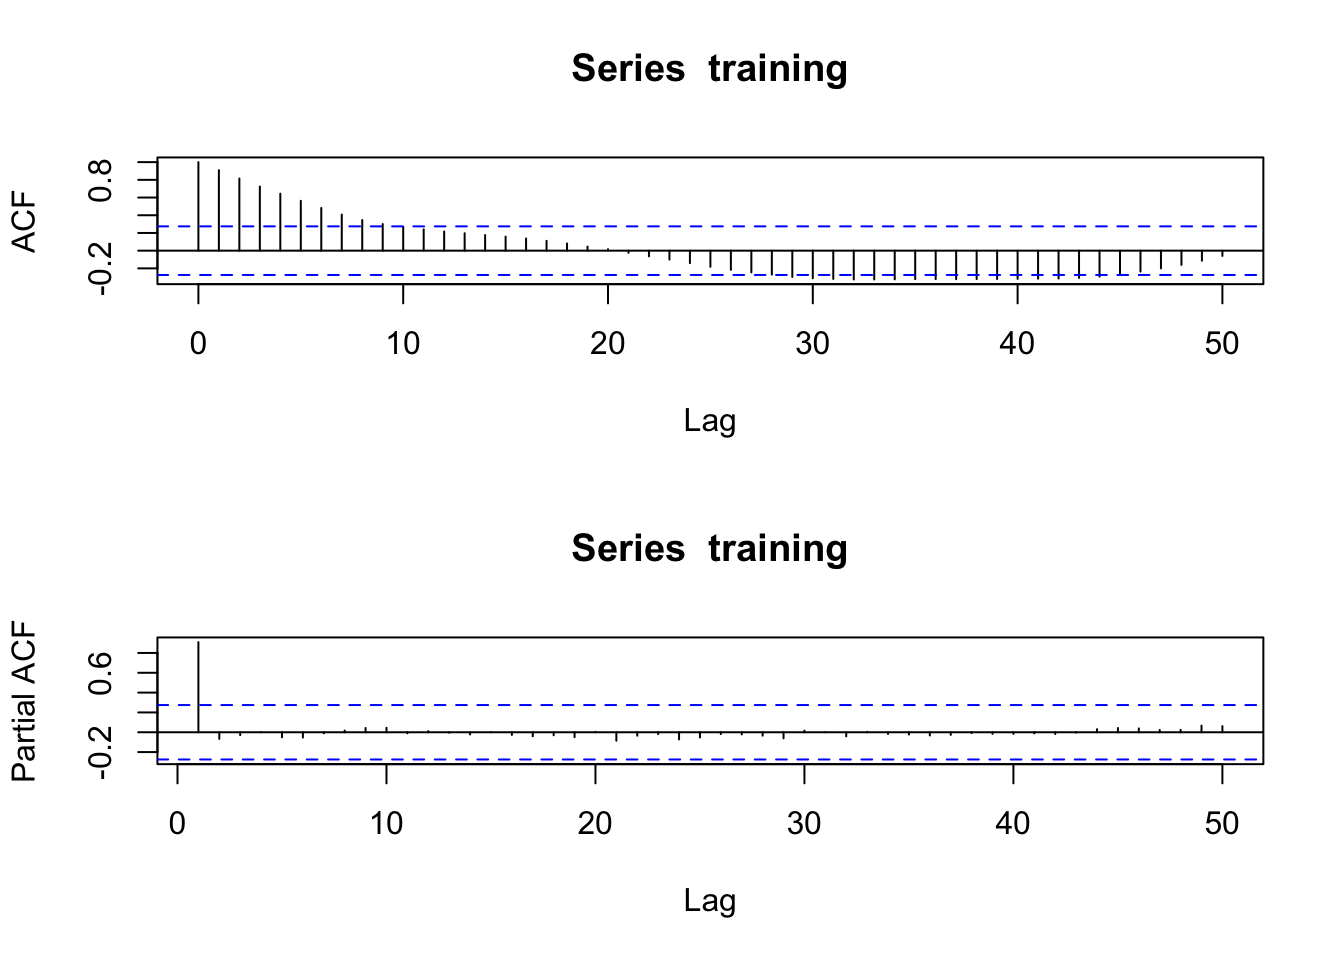
\includegraphics{Joseph-Chang---PSTAT174-Final-Project_files/figure-latex/unnamed-chunk-9-1.pdf}

\begin{Shaded}
\begin{Highlighting}[]
\FunctionTok{pacf}\NormalTok{(dat}\FloatTok{.1}\NormalTok{, }\AttributeTok{lag.max =} \DecValTok{40}\NormalTok{, }\AttributeTok{main=}\StringTok{"PACF of difference at lag 1 once"}\NormalTok{, }\AttributeTok{ylim=}\FunctionTok{c}\NormalTok{(}\SpecialCharTok{{-}}\DecValTok{1}\NormalTok{,}\DecValTok{1}\NormalTok{),}\AttributeTok{xlab=}\StringTok{"h"}\NormalTok{, }\AttributeTok{ylab=} \FunctionTok{expression}\NormalTok{(}\FunctionTok{hat}\NormalTok{(rho)[X](h)))}
\end{Highlighting}
\end{Shaded}

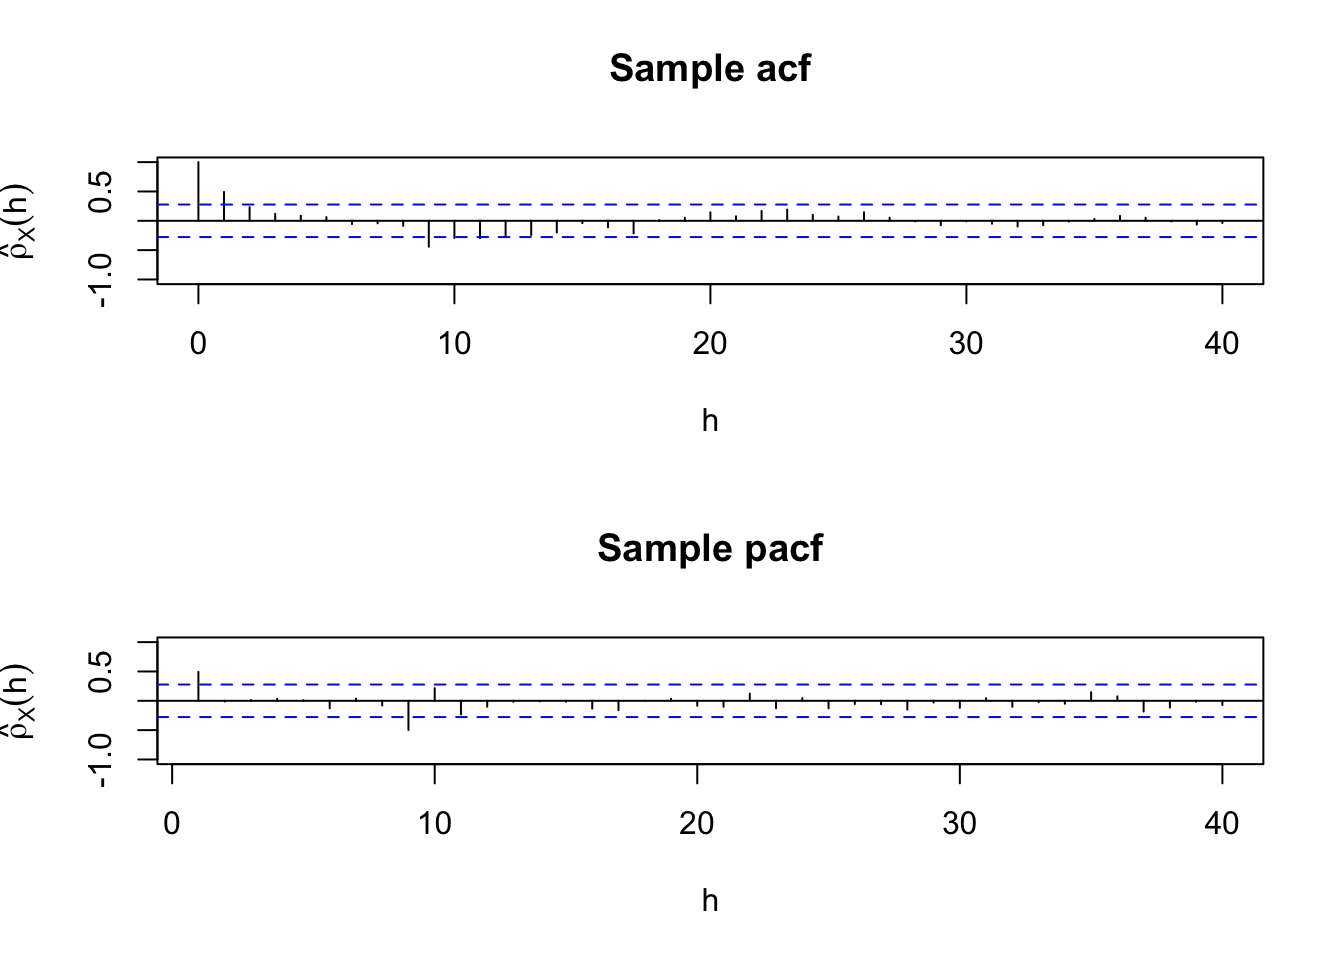
\includegraphics{Joseph-Chang---PSTAT174-Final-Project_files/figure-latex/unnamed-chunk-9-2.pdf}

From the ACF, I noticed that lags 1,9,10,11 were outside of the
confidence interval, with lag 9 being the furthest outside and as the
peak. For PACF, both lags 1 and 9 outside confidence interval, with 9
again being the furthest outside and the peak.

\hypertarget{model-estimation}{%
\section{Model Estimation}\label{model-estimation}}

Here, I will estimate the parameters on my potential model. I used a for
loop function to find the five models with the lowest AICc to run
diagnostics on. Based from the ACF of dat.1, lags 1, 9, 10, 11 were
outside the confidence interval and for PACF lags 1 and 9 were outside.
Therefore, I suspect there might be some seasonality and the potential
use of the SARIMA model, with period at 9 since both ACF and PACF had
peak at 9.

Both the ACF and PACF showed peak and outside confidence interval at lag
9 but not at lag 18. Thus in my for loop, I put values of both P and Q
in SARIMA to be either 0 or 1. In addition, p and q will also take on
the same values as P and Q (either 0 or 1) because both ACF and PACF
also showed lag 1 to be outside confidence interval.

\begin{Shaded}
\begin{Highlighting}[]
\CommentTok{\# range of parameters}
\NormalTok{df }\OtherTok{\textless{}{-}} \FunctionTok{expand.grid}\NormalTok{(}\AttributeTok{p=}\DecValTok{0}\SpecialCharTok{:}\DecValTok{1}\NormalTok{, }\AttributeTok{q=}\DecValTok{0}\SpecialCharTok{:}\DecValTok{1}\NormalTok{, }\AttributeTok{P=} \DecValTok{0}\SpecialCharTok{:}\DecValTok{1}\NormalTok{, }\AttributeTok{Q=}\DecValTok{0}\SpecialCharTok{:}\DecValTok{1}\NormalTok{)}
\NormalTok{df }\OtherTok{\textless{}{-}} \FunctionTok{cbind}\NormalTok{(df, }\AttributeTok{AICc=}\ConstantTok{NA}\NormalTok{)}

\ControlFlowTok{for}\NormalTok{ (i }\ControlFlowTok{in} \DecValTok{1}\SpecialCharTok{:}\FunctionTok{nrow}\NormalTok{(df)) \{}
\NormalTok{  sarima.obj }\OtherTok{\textless{}{-}} \ConstantTok{NULL}
  \FunctionTok{try}\NormalTok{(arima.obj }\OtherTok{\textless{}{-}} \FunctionTok{arima}\NormalTok{(training.log, }\AttributeTok{order=}\FunctionTok{c}\NormalTok{(df}\SpecialCharTok{$}\NormalTok{p[i],}\DecValTok{1}\NormalTok{, df}\SpecialCharTok{$}\NormalTok{q[i]), }\AttributeTok{seasonal =}  \FunctionTok{list}\NormalTok{(}\AttributeTok{order=}\FunctionTok{c}\NormalTok{(df}\SpecialCharTok{$}\NormalTok{P[i], }\DecValTok{0}\NormalTok{, df}\SpecialCharTok{$}\NormalTok{Q[i]), }\AttributeTok{period=}\DecValTok{9}\NormalTok{), }\AttributeTok{method=}\StringTok{"ML"}\NormalTok{))}
  \ControlFlowTok{if}\NormalTok{ (}\SpecialCharTok{!}\FunctionTok{is.null}\NormalTok{(arima.obj)) \{ df}\SpecialCharTok{$}\NormalTok{AICc[i] }\OtherTok{\textless{}{-}} \FunctionTok{AICc}\NormalTok{(arima.obj) \}}
\NormalTok{\}}

\CommentTok{\# first five models with lowest AICc}
\FunctionTok{head}\NormalTok{(df[}\FunctionTok{order}\NormalTok{(df}\SpecialCharTok{$}\NormalTok{AICc),], }\DecValTok{5}\NormalTok{)}
\end{Highlighting}
\end{Shaded}

\begin{verbatim}
##    p q P Q   AICc
## 6  1 0 1 0 -143.0
## 14 1 0 1 1 -140.9
## 8  1 1 1 0 -140.8
## 10 1 0 0 1 -138.9
## 16 1 1 1 1 -138.8
\end{verbatim}

Based from the lowest AICc, I will consider the two best models for
diagnostics.

Model 1 will be SARIMA (1,1,0),(1,0,0), period at 9 Model 2 will be
SARIMA (1,1,0),(1,0,1), period at 9.

\begin{Shaded}
\begin{Highlighting}[]
\CommentTok{\# Final model 1}
\NormalTok{fit1 }\OtherTok{\textless{}{-}} \FunctionTok{arima}\NormalTok{(training.log, }\AttributeTok{order =} \FunctionTok{c}\NormalTok{(}\DecValTok{1}\NormalTok{,}\DecValTok{1}\NormalTok{,}\DecValTok{0}\NormalTok{), }\AttributeTok{seasonal =}  \FunctionTok{list}\NormalTok{(}\AttributeTok{order=}\FunctionTok{c}\NormalTok{(}\DecValTok{1}\NormalTok{,}\DecValTok{0}\NormalTok{,}\DecValTok{0}\NormalTok{), }\AttributeTok{period=}\DecValTok{9}\NormalTok{), }\AttributeTok{method =} \StringTok{"ML"}\NormalTok{)}
\NormalTok{fit1}
\end{Highlighting}
\end{Shaded}

\begin{verbatim}
## 
## Call:
## arima(x = training.log, order = c(1, 1, 0), seasonal = list(order = c(1, 0, 
##     0), period = 9), method = "ML")
## 
## Coefficients:
##         ar1    sar1
##       0.830  -0.566
## s.e.  0.079   0.122
## 
## sigma^2 estimated as 0.00271:  log likelihood = 74.61,  aic = -143.2
\end{verbatim}

\begin{Shaded}
\begin{Highlighting}[]
\FunctionTok{AICc}\NormalTok{(fit1)}
\end{Highlighting}
\end{Shaded}

\begin{verbatim}
## [1] -143
\end{verbatim}

\begin{Shaded}
\begin{Highlighting}[]
\CommentTok{\# Final model 2}
\NormalTok{fit2 }\OtherTok{\textless{}{-}} \FunctionTok{arima}\NormalTok{(training.log, }\AttributeTok{order =} \FunctionTok{c}\NormalTok{(}\DecValTok{1}\NormalTok{,}\DecValTok{1}\NormalTok{,}\DecValTok{0}\NormalTok{), }\AttributeTok{seasonal =}  \FunctionTok{list}\NormalTok{(}\AttributeTok{order=}\FunctionTok{c}\NormalTok{(}\DecValTok{1}\NormalTok{,}\DecValTok{0}\NormalTok{,}\DecValTok{1}\NormalTok{), }\AttributeTok{period=}\DecValTok{9}\NormalTok{), }\AttributeTok{method =} \StringTok{"ML"}\NormalTok{)}
\NormalTok{fit2}
\end{Highlighting}
\end{Shaded}

\begin{verbatim}
## 
## Call:
## arima(x = training.log, order = c(1, 1, 0), seasonal = list(order = c(1, 0, 
##     1), period = 9), method = "ML")
## 
## Coefficients:
##         ar1    sar1    sma1
##       0.844  -0.502  -0.111
## s.e.  0.082   0.191   0.227
## 
## sigma^2 estimated as 0.00268:  log likelihood = 74.73,  aic = -141.4
\end{verbatim}

\begin{Shaded}
\begin{Highlighting}[]
\FunctionTok{AICc}\NormalTok{(fit2)}
\end{Highlighting}
\end{Shaded}

\begin{verbatim}
## [1] -140.9
\end{verbatim}

Both Model 1 and 2 are stationary because their phi values are less than
the absolute value of 1. Both are invertible because all AR models are
invertible.

\hypertarget{model-diagnostics-for-model-1}{%
\subsection{Model Diagnostics for model
1}\label{model-diagnostics-for-model-1}}

This will be model diagnostics for model 1: SARIMA (1,1,0),(1,0,0),
period at 9.

\begin{Shaded}
\begin{Highlighting}[]
\CommentTok{\# residual plots}
\NormalTok{res }\OtherTok{\textless{}{-}} \FunctionTok{residuals}\NormalTok{(fit1)}
\FunctionTok{mean}\NormalTok{(res)}
\end{Highlighting}
\end{Shaded}

\begin{verbatim}
## [1] 0.0139
\end{verbatim}

\begin{Shaded}
\begin{Highlighting}[]
\FunctionTok{var}\NormalTok{(res)}
\end{Highlighting}
\end{Shaded}

\begin{verbatim}
## [1] 0.002512
\end{verbatim}

\begin{Shaded}
\begin{Highlighting}[]
\CommentTok{\# layout}
\FunctionTok{par}\NormalTok{(}\AttributeTok{mfrow=}\FunctionTok{c}\NormalTok{(}\DecValTok{1}\NormalTok{,}\DecValTok{1}\NormalTok{))}
\FunctionTok{ts.plot}\NormalTok{(res, }\AttributeTok{main  =} \StringTok{"Fitted Residuals"}\NormalTok{)}
\NormalTok{t }\OtherTok{\textless{}{-}} \DecValTok{1}\SpecialCharTok{:}\FunctionTok{length}\NormalTok{(res)}
\NormalTok{fit1.res }\OtherTok{=} \FunctionTok{lm}\NormalTok{(res}\SpecialCharTok{\textasciitilde{}}\NormalTok{t)}
\FunctionTok{abline}\NormalTok{(fit1.res)}
\FunctionTok{abline}\NormalTok{(}\AttributeTok{h=}\FunctionTok{mean}\NormalTok{(res), }\AttributeTok{col =} \StringTok{"blue"}\NormalTok{)}
\end{Highlighting}
\end{Shaded}

\includegraphics{Joseph-Chang---PSTAT174-Final-Project_files/figure-latex/unnamed-chunk-13-1.pdf}

\begin{Shaded}
\begin{Highlighting}[]
\CommentTok{\# Testing independence of residuals}
\FunctionTok{Box.test}\NormalTok{(res, }\AttributeTok{lag =} \FunctionTok{sqrt}\NormalTok{(}\DecValTok{61}\NormalTok{), }\AttributeTok{type =} \FunctionTok{c}\NormalTok{(}\StringTok{"Box{-}Pierce"}\NormalTok{), }\AttributeTok{fitdf =} \DecValTok{2}\NormalTok{)}
\end{Highlighting}
\end{Shaded}

\begin{verbatim}
## 
##  Box-Pierce test
## 
## data:  res
## X-squared = 6.7, df = 5.8, p-value = 0.3
\end{verbatim}

\begin{Shaded}
\begin{Highlighting}[]
\FunctionTok{Box.test}\NormalTok{(res, }\AttributeTok{lag =} \FunctionTok{sqrt}\NormalTok{(}\DecValTok{61}\NormalTok{), }\AttributeTok{type =} \FunctionTok{c}\NormalTok{(}\StringTok{"Ljung{-}Box"}\NormalTok{), }\AttributeTok{fitdf =} \DecValTok{2}\NormalTok{)}
\end{Highlighting}
\end{Shaded}

\begin{verbatim}
## 
##  Box-Ljung test
## 
## data:  res
## X-squared = 7.4, df = 5.8, p-value = 0.3
\end{verbatim}

\begin{Shaded}
\begin{Highlighting}[]
\FunctionTok{Box.test}\NormalTok{(res}\SpecialCharTok{\^{}}\DecValTok{2}\NormalTok{, }\AttributeTok{lag =} \FunctionTok{sqrt}\NormalTok{(}\DecValTok{61}\NormalTok{), }\AttributeTok{type =} \FunctionTok{c}\NormalTok{(}\StringTok{"Ljung{-}Box"}\NormalTok{), }\AttributeTok{fitdf =} \DecValTok{0}\NormalTok{)}
\end{Highlighting}
\end{Shaded}

\begin{verbatim}
## 
##  Box-Ljung test
## 
## data:  res^2
## X-squared = 3.8, df = 7.8, p-value = 0.9
\end{verbatim}

\begin{Shaded}
\begin{Highlighting}[]
\CommentTok{\# Testing normality of residuals}
\FunctionTok{shapiro.test}\NormalTok{(res)}
\end{Highlighting}
\end{Shaded}

\begin{verbatim}
## 
##  Shapiro-Wilk normality test
## 
## data:  res
## W = 0.96, p-value = 0.06
\end{verbatim}

\begin{Shaded}
\begin{Highlighting}[]
\CommentTok{\# Histogram and qq plot of residuals}
\FunctionTok{par}\NormalTok{(}\AttributeTok{mfrow=}\FunctionTok{c}\NormalTok{(}\DecValTok{1}\NormalTok{,}\DecValTok{2}\NormalTok{))}
\FunctionTok{hist}\NormalTok{(res, }\AttributeTok{main=} \StringTok{"Histogram"}\NormalTok{)}
\FunctionTok{qqnorm}\NormalTok{(res)}
\FunctionTok{qqline}\NormalTok{(res, }\AttributeTok{col =} \StringTok{"blue"}\NormalTok{)}
\end{Highlighting}
\end{Shaded}

\includegraphics{Joseph-Chang---PSTAT174-Final-Project_files/figure-latex/unnamed-chunk-13-2.pdf}

Model 1 passes all tests and residuals are normal. Next, I will check
ACF and PACF of residuals.

\begin{Shaded}
\begin{Highlighting}[]
\CommentTok{\# ACF and PACF of residuals}
\FunctionTok{par}\NormalTok{(}\AttributeTok{mfrow=}\FunctionTok{c}\NormalTok{(}\DecValTok{1}\NormalTok{,}\DecValTok{2}\NormalTok{))}
\FunctionTok{acf}\NormalTok{(res, }\AttributeTok{main =} \StringTok{"Autocorrelation"}\NormalTok{, }\AttributeTok{lag.max =} \DecValTok{40}\NormalTok{)}
\FunctionTok{pacf}\NormalTok{(res, }\AttributeTok{main =} \StringTok{"Partial Autocorrelation"}\NormalTok{, }\AttributeTok{lag.max =} \DecValTok{40}\NormalTok{)}
\end{Highlighting}
\end{Shaded}

\includegraphics{Joseph-Chang---PSTAT174-Final-Project_files/figure-latex/unnamed-chunk-14-1.pdf}

The ACF and PACF of residuals shows no lags outside of confidence
interval. The fitted residuals are to AR(0), so it is white noise. This
passes diagnostic checking for model 1.

\hypertarget{model-diagnostics-for-model-2}{%
\subsection{Model Diagnostics for model
2}\label{model-diagnostics-for-model-2}}

This will be model diagnostics for model 2: SARIMA (1,1,0),(1,0,1),
period at 9.

\begin{Shaded}
\begin{Highlighting}[]
\CommentTok{\# residual plots}
\NormalTok{res2 }\OtherTok{\textless{}{-}} \FunctionTok{residuals}\NormalTok{(fit2)}
\FunctionTok{mean}\NormalTok{(res2)}
\end{Highlighting}
\end{Shaded}

\begin{verbatim}
## [1] 0.01364
\end{verbatim}

\begin{Shaded}
\begin{Highlighting}[]
\FunctionTok{var}\NormalTok{(res2)}
\end{Highlighting}
\end{Shaded}

\begin{verbatim}
## [1] 0.002493
\end{verbatim}

\begin{Shaded}
\begin{Highlighting}[]
\CommentTok{\# layout}
\FunctionTok{par}\NormalTok{(}\AttributeTok{mfrow=}\FunctionTok{c}\NormalTok{(}\DecValTok{1}\NormalTok{,}\DecValTok{1}\NormalTok{))}
\FunctionTok{ts.plot}\NormalTok{(res2, }\AttributeTok{main  =} \StringTok{"Fitted Residuals"}\NormalTok{)}
\NormalTok{t }\OtherTok{\textless{}{-}} \DecValTok{1}\SpecialCharTok{:}\FunctionTok{length}\NormalTok{(res2)}
\NormalTok{fit2.res }\OtherTok{=} \FunctionTok{lm}\NormalTok{(res2}\SpecialCharTok{\textasciitilde{}}\NormalTok{t)}
\FunctionTok{abline}\NormalTok{(fit2.res)}
\FunctionTok{abline}\NormalTok{(}\AttributeTok{h=}\FunctionTok{mean}\NormalTok{(res2), }\AttributeTok{col =} \StringTok{"blue"}\NormalTok{)}
\end{Highlighting}
\end{Shaded}

\includegraphics{Joseph-Chang---PSTAT174-Final-Project_files/figure-latex/unnamed-chunk-15-1.pdf}

\begin{Shaded}
\begin{Highlighting}[]
\CommentTok{\# Testing independence of residuals}
\FunctionTok{Box.test}\NormalTok{(res2, }\AttributeTok{lag =} \FunctionTok{sqrt}\NormalTok{(}\DecValTok{61}\NormalTok{), }\AttributeTok{type =} \FunctionTok{c}\NormalTok{(}\StringTok{"Box{-}Pierce"}\NormalTok{), }\AttributeTok{fitdf =} \DecValTok{3}\NormalTok{)}
\end{Highlighting}
\end{Shaded}

\begin{verbatim}
## 
##  Box-Pierce test
## 
## data:  res2
## X-squared = 6.8, df = 4.8, p-value = 0.2
\end{verbatim}

\begin{Shaded}
\begin{Highlighting}[]
\FunctionTok{Box.test}\NormalTok{(res2, }\AttributeTok{lag =} \FunctionTok{sqrt}\NormalTok{(}\DecValTok{61}\NormalTok{), }\AttributeTok{type =} \FunctionTok{c}\NormalTok{(}\StringTok{"Ljung{-}Box"}\NormalTok{), }\AttributeTok{fitdf =} \DecValTok{3}\NormalTok{)}
\end{Highlighting}
\end{Shaded}

\begin{verbatim}
## 
##  Box-Ljung test
## 
## data:  res2
## X-squared = 7.5, df = 4.8, p-value = 0.2
\end{verbatim}

\begin{Shaded}
\begin{Highlighting}[]
\FunctionTok{Box.test}\NormalTok{(res2}\SpecialCharTok{\^{}}\DecValTok{2}\NormalTok{, }\AttributeTok{lag =} \FunctionTok{sqrt}\NormalTok{(}\DecValTok{61}\NormalTok{), }\AttributeTok{type =} \FunctionTok{c}\NormalTok{(}\StringTok{"Ljung{-}Box"}\NormalTok{), }\AttributeTok{fitdf =} \DecValTok{0}\NormalTok{)}
\end{Highlighting}
\end{Shaded}

\begin{verbatim}
## 
##  Box-Ljung test
## 
## data:  res2^2
## X-squared = 3.7, df = 7.8, p-value = 0.9
\end{verbatim}

\begin{Shaded}
\begin{Highlighting}[]
\CommentTok{\# Testing normality of residuals}
\FunctionTok{shapiro.test}\NormalTok{(res2)}
\end{Highlighting}
\end{Shaded}

\begin{verbatim}
## 
##  Shapiro-Wilk normality test
## 
## data:  res2
## W = 0.96, p-value = 0.07
\end{verbatim}

\begin{Shaded}
\begin{Highlighting}[]
\CommentTok{\# Histogram and qq plot of residuals}
\FunctionTok{par}\NormalTok{(}\AttributeTok{mfrow=}\FunctionTok{c}\NormalTok{(}\DecValTok{1}\NormalTok{,}\DecValTok{2}\NormalTok{))}
\FunctionTok{hist}\NormalTok{(res2, }\AttributeTok{main=} \StringTok{"Histogram"}\NormalTok{)}
\FunctionTok{qqnorm}\NormalTok{(res2)}
\FunctionTok{qqline}\NormalTok{(res2, }\AttributeTok{col =} \StringTok{"blue"}\NormalTok{)}
\end{Highlighting}
\end{Shaded}

\includegraphics{Joseph-Chang---PSTAT174-Final-Project_files/figure-latex/unnamed-chunk-15-2.pdf}

Model 2 passes all tests and residuals are normal. Next, I will check
ACF and PACF of residuals.

\begin{Shaded}
\begin{Highlighting}[]
\CommentTok{\# ACF and PACF of residuals}
\FunctionTok{par}\NormalTok{(}\AttributeTok{mfrow=}\FunctionTok{c}\NormalTok{(}\DecValTok{1}\NormalTok{,}\DecValTok{2}\NormalTok{))}
\FunctionTok{acf}\NormalTok{(res2, }\AttributeTok{main =} \StringTok{"Autocorrelation"}\NormalTok{, }\AttributeTok{lag.max =} \DecValTok{40}\NormalTok{)}
\FunctionTok{pacf}\NormalTok{(res2, }\AttributeTok{main =} \StringTok{"Partial Autocorrelation"}\NormalTok{, }\AttributeTok{lag.max =} \DecValTok{40}\NormalTok{)}
\end{Highlighting}
\end{Shaded}

\includegraphics{Joseph-Chang---PSTAT174-Final-Project_files/figure-latex/unnamed-chunk-16-1.pdf}

The ACF of residuals shows no lags outside, but PACF does show one lag
barely outside of the confidence interval. This results in in model 2
failing diagnostic checking.

\hypertarget{best-model}{%
\subsection{Best model}\label{best-model}}

Since the analysis of residuals in model 1 was satisfactory and passed
diagnostic checking, I will use fit1.

\begin{Shaded}
\begin{Highlighting}[]
\NormalTok{fit1}
\end{Highlighting}
\end{Shaded}

\begin{verbatim}
## 
## Call:
## arima(x = training.log, order = c(1, 1, 0), seasonal = list(order = c(1, 0, 
##     0), period = 9), method = "ML")
## 
## Coefficients:
##         ar1    sar1
##       0.830  -0.566
## s.e.  0.079   0.122
## 
## sigma^2 estimated as 0.00271:  log likelihood = 74.61,  aic = -143.2
\end{verbatim}

The final model can be written as
\((1-0.83B)(1+0.566B^9)(1-B)X_t = Z_t, Z_t \sim WN(0, 0.00271)\)

\hypertarget{data-forecasting}{%
\subsection{Data Forecasting}\label{data-forecasting}}

In the final step of forecasting, I will predict 10 future observations
(colored in red) and plot it against the testing set of the original
data (colored in blue) for comparison. Then, I will do the same for the
transformed data. For fun, I predicted 5 years my prediction in the
original data.

\begin{Shaded}
\begin{Highlighting}[]
\CommentTok{\# Predict 15 future observations on data and plot on original}
\NormalTok{m }\OtherTok{\textless{}{-}} \FunctionTok{length}\NormalTok{(training)}
\NormalTok{mypred }\OtherTok{\textless{}{-}} \FunctionTok{predict}\NormalTok{(fit1, }\AttributeTok{n.ahead=}\DecValTok{15}\NormalTok{)}

\FunctionTok{ts.plot}\NormalTok{(training, }\AttributeTok{xlim=}\FunctionTok{c}\NormalTok{(}\DecValTok{1}\NormalTok{, }\FunctionTok{length}\NormalTok{(training)}\SpecialCharTok{+}\DecValTok{15}\NormalTok{), }\AttributeTok{ylim=}\FunctionTok{c}\NormalTok{(}\FunctionTok{min}\NormalTok{(training), }\DecValTok{1000}\NormalTok{) , }\AttributeTok{xlab =} \StringTok{"Years after 1960"}\NormalTok{, }\AttributeTok{ylab =} \StringTok{"Billions of USD"}\NormalTok{)}

\FunctionTok{points}\NormalTok{((m}\SpecialCharTok{+}\DecValTok{1}\NormalTok{)}\SpecialCharTok{:}\NormalTok{(m}\SpecialCharTok{+}\DecValTok{15}\NormalTok{), }\AttributeTok{col=}\StringTok{"blue"}\NormalTok{, }\FunctionTok{exp}\NormalTok{(mypred}\SpecialCharTok{$}\NormalTok{pred))}
\FunctionTok{points}\NormalTok{((m}\SpecialCharTok{+}\DecValTok{1}\NormalTok{)}\SpecialCharTok{:}\NormalTok{(m}\SpecialCharTok{+}\DecValTok{10}\NormalTok{), }\AttributeTok{col=}\StringTok{"red"}\NormalTok{, testing)}
\FunctionTok{lines}\NormalTok{((m}\SpecialCharTok{+}\DecValTok{1}\NormalTok{)}\SpecialCharTok{:}\NormalTok{(m}\SpecialCharTok{+}\DecValTok{10}\NormalTok{), }\AttributeTok{col=}\StringTok{"black"}\NormalTok{, testing, }\AttributeTok{lty=} \StringTok{"solid"}\NormalTok{)}
\FunctionTok{lines}\NormalTok{((}\FunctionTok{exp}\NormalTok{(mypred}\SpecialCharTok{$}\NormalTok{pred }\SpecialCharTok{+}\DecValTok{2}\SpecialCharTok{*}\NormalTok{mypred}\SpecialCharTok{$}\NormalTok{se)), }\AttributeTok{col =} \StringTok{"blue"}\NormalTok{, }\AttributeTok{lty=} \StringTok{"dashed"}\NormalTok{)}
\FunctionTok{lines}\NormalTok{((}\FunctionTok{exp}\NormalTok{(mypred}\SpecialCharTok{$}\NormalTok{pred }\SpecialCharTok{{-}}\DecValTok{2}\SpecialCharTok{*}\NormalTok{mypred}\SpecialCharTok{$}\NormalTok{se)), }\AttributeTok{col =} \StringTok{"blue"}\NormalTok{, }\AttributeTok{lty=} \StringTok{"dashed"}\NormalTok{)}
\end{Highlighting}
\end{Shaded}

\includegraphics{Joseph-Chang---PSTAT174-Final-Project_files/figure-latex/unnamed-chunk-18-1.pdf}

\begin{Shaded}
\begin{Highlighting}[]
\CommentTok{\# predict 10 future observations and plot on transformed data}
\NormalTok{m }\OtherTok{\textless{}{-}} \FunctionTok{length}\NormalTok{(training.log)}
\NormalTok{mypred }\OtherTok{\textless{}{-}} \FunctionTok{predict}\NormalTok{(fit1, }\AttributeTok{n.ahead=}\DecValTok{10}\NormalTok{)}

\FunctionTok{ts.plot}\NormalTok{(training.log, }\AttributeTok{xlim=}\FunctionTok{c}\NormalTok{(}\DecValTok{1}\NormalTok{, }\FunctionTok{length}\NormalTok{(training.log)}\SpecialCharTok{+}\DecValTok{10}\NormalTok{), }\AttributeTok{ylim=}\FunctionTok{c}\NormalTok{(}\FunctionTok{min}\NormalTok{(training.log), }\FunctionTok{max}\NormalTok{(mypred}\SpecialCharTok{$}\NormalTok{pred }\SpecialCharTok{+}\DecValTok{2}\SpecialCharTok{*}\NormalTok{mypred}\SpecialCharTok{$}\NormalTok{se)) , }\AttributeTok{xlab =} \StringTok{"Years after 1960"}\NormalTok{, }\AttributeTok{ylab =} \StringTok{"Billions of USD"}\NormalTok{)}

\FunctionTok{points}\NormalTok{((m}\SpecialCharTok{+}\DecValTok{1}\NormalTok{)}\SpecialCharTok{:}\NormalTok{(m}\SpecialCharTok{+}\DecValTok{10}\NormalTok{), }\AttributeTok{col=}\StringTok{"blue"}\NormalTok{, mypred}\SpecialCharTok{$}\NormalTok{pred)}
\FunctionTok{lines}\NormalTok{((mypred}\SpecialCharTok{$}\NormalTok{pred }\SpecialCharTok{+}\DecValTok{2}\SpecialCharTok{*}\NormalTok{mypred}\SpecialCharTok{$}\NormalTok{se), }\AttributeTok{col =} \StringTok{"blue"}\NormalTok{, }\AttributeTok{lty=} \StringTok{"dashed"}\NormalTok{)}
\FunctionTok{lines}\NormalTok{((mypred}\SpecialCharTok{$}\NormalTok{pred }\SpecialCharTok{{-}}\DecValTok{2}\SpecialCharTok{*}\NormalTok{mypred}\SpecialCharTok{$}\NormalTok{se), }\AttributeTok{col =} \StringTok{"blue"}\NormalTok{, }\AttributeTok{lty=} \StringTok{"dashed"}\NormalTok{)}
\end{Highlighting}
\end{Shaded}

\includegraphics{Joseph-Chang---PSTAT174-Final-Project_files/figure-latex/unnamed-chunk-18-2.pdf}

seasonality was there, but the period might have been wrong.

\hypertarget{conclusion}{%
\subsection{Conclusion}\label{conclusion}}

Model 1 passed diagnostic checking but Model 2 failed. Ultimately, my
predicted model followed closely with the actual model at first, but
then predicted in a different direction towards the end of the actual
data. My model correctly predicted a seasonality, but the period might
have been different. Instead of a period at 9, another period to try
could be at 10 or 11, as shown in the ACF and PACF of dat.1. The goal of
creating a model that could predict future values of the original model
was achieved. Although overall the model did correctly follow the points
in the testing set in the short-term future, predicting points in the
long-term future was not as accurate. Therefore, I would be hesitant to
use my predicted model to predict the defense budget in 10-20 years. My
model consisted of this formula : (1−0.831B)(1+0.566B\^{}9)(1−B)Xt = Zt.
I would like to acknowledge Raisa Feldman, Youhong Lee, and Sunpeng Duan
for their contributions and assistance with this project and thank them
for taking the time, effort, and energy out of their busy schedules to
help me.

\hypertarget{references}{%
\subsection{References}\label{references}}

I used this site to obtain my original dataset:
\url{https://www.kaggle.com/brandonconrady/us-military-spending-by-year-1960-2020/version/1}

\hypertarget{appendix}{%
\subsection{Appendix}\label{appendix}}

\end{document}
